% !TEX encoding = UTF-8 Unicode
% !TEX program = pdflatex
% !TEX spellcheck = en_US


% In order to correctly compile this document,
% execute the following commands:
% 1. pdflatex
% 2. pdflatex
% 3. pdflatex



\documentclass[amsthm,ebook]{saparticle}

% IF YOU USE PDFLATEX
\usepackage[utf8x]{inputenc}
% if you write in english and in greek
\usepackage{ucs}
\usepackage[greek,english]{babel}
\languageattribute{greek}{polutoniko}

% IF YOU USE XELATEX
%\usepackage{polyglossia}
% if you write in italian
%\setmainlanguage{italian}
% If you want put some ancient greek:
%\setotherlanguage[variant=polytonic]{greek}
%\newfontfamily{\greekfont}[Ligatures=TeX]{Palatino Linotype}

% dummy text (remove in a normal thesis)
% remove if not necessary
\usepackage{siunitx}
%Natbib for bibliography management
\usepackage[authoryear]{natbib}
% custom commands
\newcommand{\bs}{\textbackslash}

%%%%%%%%
%TITLE:%
%%%%%%%%
\title{Integration of Multimedia Collections and Tools
for Interaction with Digital Content.
The case study of the Archaia Kypriaki Grammateia Digital Corpus}
\author[cyi]{Valentina Vassallo\corref{first}}
\author[cyi]{Uros Damnjanovic}
\author[cyi]{Sorin Hermon}
\date{2015-11-26}
\cortext[first]{Corresponding author. Email: (u.damnjanovic, v.vassallo, s.hermon@cyi.ac.cy}
\begin{document}


\maketitle
\begin{abstract}
Supporting a discovery, use, and navigation of digital collections is a fundamental part of providing access and
encouraging inquiry, interpretation, and knowledge. In this paper we present our efforts to store and explore
multimedia collections of archaeological data. Particularly, the case study of the Archaia Kypriaki Grammateia
epigraphic collection is presented. Our work can be seen twofold. One aspect of our work is to provide a place where
the data coming from various sources can be stored and accessed. Another aspect is to provide users with means to explore
this data. We argue that currently digital libraries are constrained by their webpage-based paradigm, thus not
providing the means for utilizing the full potential of the heritage data.
\end{abstract}
\keywords{Digital libraries, Data repository, Epigraphy, User interfaces, Data visualization, Interaction}

\section{The world going digital}


\noindent Nowadays digital information format found its ways to all the spheres of our lives. Cultural heritage is no exception to
this. Gigabytes of data are being created on an every-day basis. For some time now, digital libraries are used to store
and provide access to digital heritage data. However, existing digital libraries often fail to provide the ability to
iteratively explore items, compare data trends, and engender the wisdom that comes from exploring data in new ways.
Current digital libraries are limited by their inadequate webpage-based paradigm, and it is easy for even the most
experienced scholar to get lost \citep{augmenting_2009}.
To overcome this issue, a new generation of digital
libraries should emerge that will serve as an interactive knowledge environment in which knowledge is created by
interacting with the data. Digital collections often lack features for deeper quantitative and qualitative analysis,
and even very useful functions, such as the ability to annotate or bookmark content, are often not supported. After
digitisation, these collections are typically monolithic, difficult to navigate, and can contain text which is of
variable quality in terms of language, spelling, punctuation and consistency of terminology. 

According to \citet{fast_interaction_2010} digital libraries are seen as a store of epistemic potential with interaction having
the role to reveal much of the hidden complexity. In \citet{buchel_making_2014} the authors demonstrated the role that a
set of interactions can play in supporting users' understanding of spaces and their formation of cognitive maps when
working with map-based visualisations. According to \citet{algee_viewshare_2012} interactive visualizations empower users to
discover meaning and patterns within digital collections using dynamic, interactive displays. One example of utilizing
the interactive graphics in a real world digital library is presented in \citet{hienert_integrating_2012}. Authors developed
interactive visualization tools that support exploration of search queries and search results and help users in
formulating new queries. Another example, the application called DaisyViz shown in \citet{ren_daisyviz:_2010}, tries to help
users acquire better insights of the data by enabling users to rapidly develop domain-specific information
visualizations without traditional programming. In \citet{nasar_conceptual_2011} authors proposed a conceptual framework that
uses interactive visualizations for managing personal collections of images and videos with focus on data re-finding
and improved filtering. INVISQUE \citep{wong_invisque:_2011} is a novel system designed for interactive information
exploration. Instead of a conventional list-style arrangement, in INVISQUE information is represented by a
two-dimensional spatial canvas, with each dimension representing user-defined semantics. Search results are presented
as index cards, ordered in both dimensions. Intuitive interactions are used to perform tasks such as keyword searching,
results browsing, categorizing, and linking to online resources such as Google and Twitter. An approach for
overview-first exploration of data collections based on user-selected metadata properties is presented in \citet{bernard_content-based_2012}. In a 2D layout representing entities of the selected property are laid out based on their similarity with
respect to the underlying data content. The display is enhanced by compact summarizations of underlying data elements,
and forms the basis for exploratory navigation of users in the data space. In \citet{cao_whisper:_2012} authors propose a
novel visual design termed ``Whisper'' to fulfil the need for tracing information diffusion processes in social media, in
a real time manner. BirdVis \citep{ferreira_birdvis:_2011} leverages visualization techniques and uses them in a novel way to
better assist users in the exploration of interdependencies among model parameters. Furthermore, the system allows for
comparative visualization through coordinated views, providing an intuitive interface to identify relevant correlations
and patterns. 




\section{``A place where the past meets the future'': the STARC repository}


\noindent STARC repository was initially developed to store the data coming from the daily work of the research group and as
content aggregator for various digital libraries projects: data from archaeological excavations, museums artefacts,
epigraphic corpora, etc. Data stored in the repository ranges from high resolution images, 3D models, texts, maps,
videos and audio resulting from various data acquisition procedures such as photogrammetry, laser scanning, 3D
modeling, photography, sketching, drawing and so on. \ Every item in the repository is described using a metadata
schema that depends on the type of data and according to the needs of the project. For most of the items, we are using
our own metadata schema (STARC metadata schemas) \citep{ronzino_metadata_2012, vassallo_revealing_2013}, that was developed to
thoroughly describe various aspects of data creation process. \ Once data is uploaded and available, it can also be
used in different systems. For example, the repository serves as source of data for aggregation procedures by which our
data feed the Europeana portal (\url{http://www.europeana.eu/portal/}) through different digital libraries projects (e.g.
Athena, CARARE, Linked Heritage, AthenaPlus, EAGLE). In order to facilitate the migration of data from heterogeneous
sources, the repository provides ingestion capabilities, that enable easy transfer of data from any available data
end-point. Another aspect of the back-end is the user management. It deals with providing different access levels for
different users’ groups. It also manages personal user space, where users can add their own information to the
repository and have access to it when exploring the data. Data annotations and personal collections are some of the
examples of how users can add information to the repository and use it for data exploration. 




\subsection{Tools for accessing data }


\noindent We wanted to provide users with a number of tools that they can use while exploring the repository. In traditional web
based system, navigating from one tool to another usually means that we click on a link and then move to another page
where the tool is available. Once the user is on a page s/he can start interacting with the tool by adding or modifying
data or by performing any action relevant to the selected functionality. The process of exploring the repository starts
by running the initial query (Fig.~\ref{fig:1}). 


\begin{figure}[!hbp]
\centering
 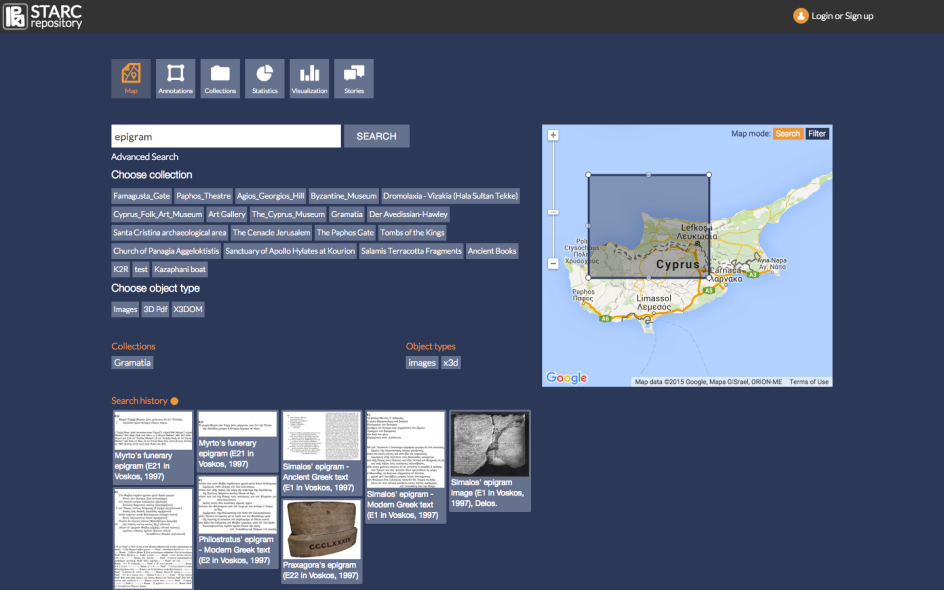
\includegraphics[width=\columnwidth]{DamnjanovicetalEAGLE2016-img001.png}
\caption{The exploration process starts by running the search. Once the results are available the user can add or remove
exploration tools. By default map tool is present in the view. The map tool is used to mark the geo-referenced data on
the map, and also to perform geo-search by defining the region of interest. }
\label{fig:1}
\end{figure}


Once the results are returned and displayed, the exploration process can start. By default the map functionality is
available in the view. When a new tool is added to the screen, it automatically gets an access to all the data
available in the current search. It also gets notified on any other tools that might be active in the view, so the
necessary communication channels are established. Once the results are ready, there are a number of filters available to
filter out the data, either by data type, collection. Search form can be used to filter out the data by typing the text
used to filter the data. As the user types, the data is automatically updated to show only those items that are related
to the text in the search field. 


\begin{figure}[!hbp]
\centering
 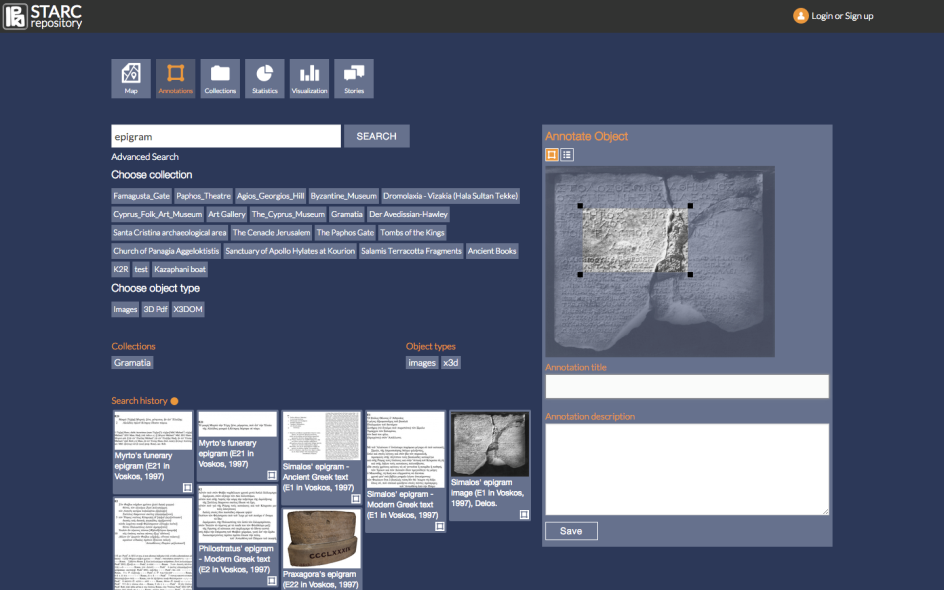
\includegraphics[width=\columnwidth]{DamnjanovicetalEAGLE2016-img002.png}
\caption{The annotation tool. The user first selects the object in the search results, then selects the region of the
object and then adds the annotation. The annotation can be accessed when the annotated object is accessed, and by
specifying in the search that the search should also include annotations. }
\label{fig:2}
\end{figure}

The user can then run a new search repeatedly, and the search history functionality
will store all those searches for later reference. The map tool (Fig.~\ref{fig:1}) is used to show information about the
geo-referenced data. It provides two main functions. One is that it accompanies the search tool. Whenever the new
search is ran, and the results become available, the map tool updates itself with new data, showing the geographical distribution of the search results. The user can then use the map to filter out the data by clicking on the
markers on the map. Also the map can also be used as a search tool. By selecting the search map mode, the rectangle
mask appears on the map, that is used to define the region of interest on the map. This region is then used as an
additional parameter for the search. 



Annotation tool is used to attach the information to the objects in the repository and share it with other users, or use
it to facilitate more efficient search. The tool is used by selecting object from search results, then either by
selecting a region in the image files (Fig.~\ref{fig:2}), or by selecting a point for 3D models, and by adding textual description
of the selected part. 


Once the search results are available, and the user selects the collection tool, the user can start adding and removing
the objects from the collection. Finally the collection is described and saved. Same as for the annotations, the
collection information is saved in the user’s personal space, and can be also used in search, by specifying to the
search that it should include the personal collections in the search. This means that the search will look not only for
objects descriptions and metadata, but will also look inside collection descriptions to try and match the query. 

In order to help in exploring the datasets, there are statistics and visualization tools. Statistics tool shows the
basic properties of the repository. A visualisation tool is used to accompany the search tool (Fig.~\ref{fig:3}). Story creation
tool is another tool that supports collaborative user generated content. It provides users with an online document
editor, where users can write their own ideas, notes, insights about the data. The document created in this way is
stored in the repository and can be accessed in the personal workspace, and shared with the others. 




\begin{figure}[!hbp]
\centering
 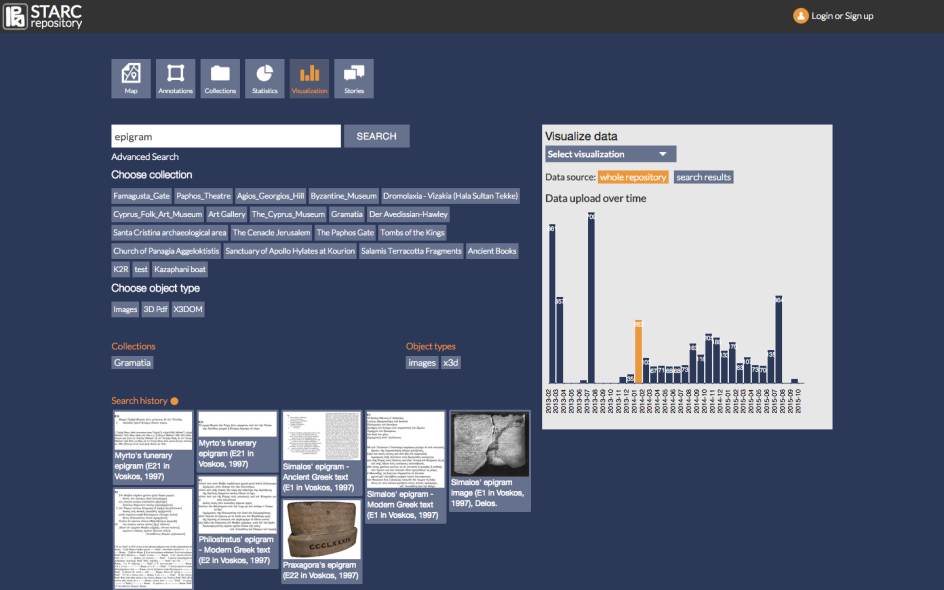
\includegraphics[width=\columnwidth]{DamnjanovicetalEAGLE2016-img003.png}
\caption{Visualization tool. Visualization tool is used to accompany the search tool by showing live visualizations as
the search results change. When the search is ran and the search results are available the visualization tools
automatically update itself and shows the visualisation related to the current search results. }
\label{fig:3}
\end{figure}




\section{Archaia Kypriaki Grammateia, the STARC Repository and the EAGLE infrastructure}


\noindent One of the most interesting collection stored in the repository is the Archaia Kypriaki Grammateia Digital Corpus
\citep{pitzalis_building_2012}. The collection is composed of Ancient Greek and Latin epigraphic texts produced within a time
span of circa 13 centuries (from the 7th century BC to the 6th century AD). The texts are attributed to Cypriot authors
or were produced in Cyprus. The corpus consists mainly of funerary or dedicatory epigrams published with their
translation in Modern Greek, critical apparatus and philological comments \citep{voskos__1997}. 

The peculiarity of the digital collection consists in the fact that, beyond the epigraphic texts, it is composed of a
series of multimedia digital resources that describe the content in a multidisciplinary way: digital texts, images
related to the epigraphic supports, 3D representation of the inscriptions, video, audio files, and so forth (Fig.~\ref{fig:4}).




\begin{figure}[!hbp]
\centering
 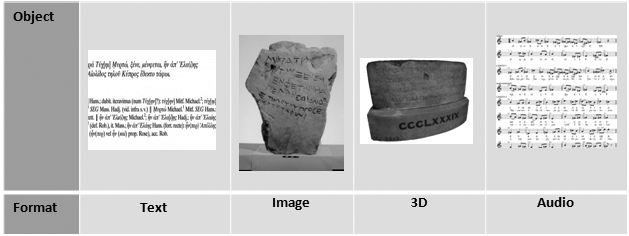
\includegraphics[width=\columnwidth]{DamnjanovicetalEAGLE2016-img004.jpg}
\caption{Multimedia data constituting the AKG digital collection stored in the STARC repository.}
\label{fig:4}
\end{figure}

Such a material needs to be described in the right way, in order to provide detailed information about all the elements
that constitute the collection. For this reason a specific metadata schema has been developed: it covers the
multidisciplinary research carried out on this material in a manner that users comprehend the complexity of such an
approach through access to heterogeneous types of information \citep{vassallo_revealing_2013}.

The metadata schema for Ancient Cypriot inscriptions integrates multidisciplinary information regarding the objects and
their multiple digital resources. It is the result of a research line developed within the group \citep{liuzzo_networking_2014} and of the assessment and comparisons of schemas, models and ontologies already in use in the digital epigraphy
field (e.g. TEI Epidoc, Dublin Core, CIDOC-CRM). 

The metadata schema is organized in groups corresponding to different research areas clustered in wrappers and
sub-wrappers, in order to fully describe all information that the ‘asset inscription’ contains. This schema,
distinguished by its multidisciplinary structure, include all disciplines relevant for description and representation
of epigraphies: archaeology (investigating for example the context of the finds), philology s(analyzing the text, the
writing style, the scripture), chemistry and geology (providing details on the material upon which inscriptions were
carved), conservation (giving information about the state of the artefact), visualization and museology (about the
museums and places of conservation).

Besides the inscriptions, since the Cypriot collection consists of their digital representations (pictures, 3D models of
inscriptions, videos, etc.), the metadata schema takes into consideration their descriptive features, their digital
provenance and other related information. For example, through the metadata it is possible to describe the digital
provenance of the 3D model of an inscription and to give information about the acquisition phase (the technique, the
tool used, the specification of the tool, the specification of the output, etc.) the post-processing (the operative
info, the file specifications, etc.) and the digital output (data format, software), according to the digital resource
obtained (Fig.~\ref{fig:5}).

The metadata schema for ancient Cypriot inscriptions aims at the following goals:

\begin{itemize}
\item to describe in detail the digital resources and its digital provenance, 
\item to provide related information about the context of the inscription, 
\item to enable harvesting to larger initiatives (e.g. Europeana, Ariadne).
\end{itemize}



\begin{figure}[!hbp]
\centering
 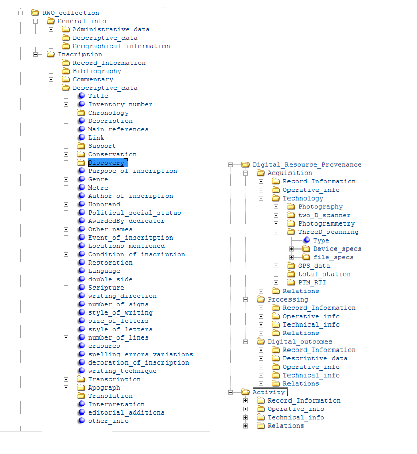
\includegraphics[width=\columnwidth]{DamnjanovicetalEAGLE2016-img005.pdf}
\caption{Diagram of the metadata schema components and relationships.}
\label{fig:5}
\end{figure}
  
  
\subsection{From STARC Repository to EAGLE infrastructure}


Beyond the functionalities developed for an enhanced users’ access to the content, the STARC repository plays as
aggregator for different digital libraries projects that in turn provide content to Europeana portal. The epigraphic
content of the Archaia Kypriaki Grammateia digital corpus is ingested through the EAGLE Project. 

The ``Europeana network of Ancient Greek and Latin Epigraphy'', is an EU funded project under the umbrella of the CIP-Best
Practice Network and whose aim is to bring together some of the most prominent European institutions and cultural
archives in the field of Classical Latin and Greek epigraphy. One of the aim is to provide Europeana with a
comprehensive collection of unique and curated online edition of historical and archaeological sources.

To encode inscriptions from different epigraphic databases, \ EAGLE developed a metadata format that assessed the
provider’s metadata structures and considered two sets of standards: TEI EpiDoc and CIDOC CRM. EpiDoc allows a full
description of the text of inscriptions while CIDOC CRM enables a further full description object-oriented,
reflecting at the same time the different souls of Epigraphy, the philological and the archaeological one. Content
providers use different models according to the fact their databases are more oriented towards the text of an
inscription or towards the archaeological object that bears the text. According to the epigraphers’ community needs,
EAGLE consortium developed the data model on the base of the two sets of standards \citep{liuzzo_networking_2014}. Finally, the
EAGLE data model is mapped to the Europeana Data Model (EDM), in order to be ingested into the Europeana portal.

The content provided by the EAGLE consortium, due to the transformation into the EAGLE metadata model, produce three
different groups of metadata according to the digital objects they are connected to: artefacts, documental
manifestation, visual representation. The data that are sent to Europeana belong to the category of the artefacts (the
inscriptions represented as texts, called by Europeana ``Cultural Heritage Object'' - CHO) and of the visual
representation (the images related to the inscriptions, called by Europeana ``WebResource''). The distinction between CHO
and WebResource has been introduced in Europeana as a result of the introduction of the new EDM schema to provide the
users with a better navigation and data retrieval and to aggregate under the same umbrella all the resources available
for a Cultural Heritage Object, avoiding data duplication in the portal.

Most of the consortium data, as well as the majority of the existent epigraphic databases worldwide, are compliant to
Epidoc. This allows to perform a smooth mapping to the EAGLE data model, to have results that are aligned to the
project aims (e.g. the possibility to create dedicated groups of metadata associated with the category of the object)
and to simplify the involvement of other databases in EAGLE through the enlargement of the consortium.

As previously mentioned, the Archaia Kypriaki Grammateia digital corpus data integrated in the STARC Repository are
different from other epigraphic databases data. The study of the epigraphy is not text-centric. The text is one of the
representations of the artefact: the archaeological object, the support, the 2D image or the 3D of the object are all
resources that, even if connected, have their own identity and their own set of information. Moreover, the AKG is a
collection of texts accompanied by their translations, notes and commentaries as published in its last edition by
Voskos \citep{voskos__1997}, therefore it is a digital form of this important editorial printed work, to which are connected
all a series of digital resources that help to enrich the corpus.

Such a material and the metadata schema used for the description of this content converges in a difficulty to map our
metadata schema to EAGLE data model. This implies a further effort to integrate the content into the EAGLE
infrastructure for a compliant visualization with the other content and retrieval in the EAGLE and Europeana portals.
Concerning the issues connected to the mapping and integration of the AKG data into EAGLE portal, possible solutions
have been investigated and are currently under tests:

\begin{itemize}
\item the creation and use of relations that are able to aggregate all the resources under a specific resource
identified as reference item.
\item the creation of rules for the development of a script that will be able to map to the Eagle data model every time
according to the type of object we are dealing with. This implies also an editing of the metadata, creating single
items that have as head the information about the inscription (e.g. the Ancient Greek text) and to which are attached
all the other metadata sets concerning the related objects (e.g. the Modern Greek text, the image support of the
inscription, the commentary, the 3D of the support-inscription, etc.).
\end{itemize}
Even if the first solution would be much faster from a technical point of view, at the moment is under preparation a
test for the second solution. In fact the latter, even if it is time-consuming in terms of elaboration, seems to be the
best solution for avoiding data duplication and for having more cohesive data. 

\section{Conclusions}


We presented in this paper a digital data repository and showed number of innovative tools used to access and explore
its collections. One of the most interesting collection stored in the repository is the Archaia Kypriaki Grammateia
Digital Corpus composed of Ancient Greek and Latin epigraphic texts. We argued that by interacting with data in an
innovative ways can help users better understand data and stimulate knowledge creation. With the set of proposed
functionalities we also enabled exploration of the epigraphic text in a way that supports sense making, understanding
and collaboration. We also showed how the collection of epigraphic texts can be used within other projects by mapping
our data to the appropriate data formats. Next step is to set up an evaluation framework that will try to measure and
evaluate the contribution of each tool to the users daily tasks. We want to measure the benefits of using such a tools
by performing various evaluation tasks and measuring the user's performance. 


\bibliographystyle{sapauth-eng}
\bibliography{../../EAGLE}

\end{document}